%%%%%%%%%%%%%%%%%%%%%%%%%%%%%%%%%%%%%%%%%%%%%%%%%%%%%%%%%%%%%%%%%%%%%%%%%%%%%%%%
% simulation.tex: Chapter on MC production:
%%%%%%%%%%%%%%%%%%%%%%%%%%%%%%%%%%%%%%%%%%%%%%%%%%%%%%%%%%%%%%%%%%%%%%%%%%%%%%%%
\chapter{Experiment Simulation}
\label{simulation_chapter}
Typical analyses using the CMS detector rely on detailed simulations of the physics processes and particle reconstruction within each event to compare with observations in data in order to measure properties of the standard model or find variations from expectation that could be caused by new physics.
The standard tool used to produce these simulations is the Monte Carlo (MC) method, where the detector and potential initial states are used with random number generators to individually simulate full events.
By producing large numbers of individual events, the underlying distributions of the observables can be determined and compared to data, and modifications to the available physics can be added to find the expected impact of any given physics model.

Many inputs are required to produce accurate simulations of CMS events.
First, the initial proton collision must be simulated for the process of interest, as well as its resulting decay into observable particles, generally referred to as the generation step.
Then passage and resulting interactions of the collision products with the CMS detector must be simulated, itself a fundamentally quantum and probabilistic process, as well as the response of the detector to these interactions, together known as the simulation step.
Lastly the detector responses are transformed into the digital formats used in the real detector so that identical reconstruction algorithms can be applied to the simulation and data, known as the digitization step.

Due to the complexity and importance of these simulations much of the underlying technique is shared between analyses, and several techniques for correcting the simulations to better match data that have been developed are applied here. 


%%%%%%%%%%%%%%%%%%%%%%%%%%%%%%%%%%%%%%%%%%%%%%%%%%%%%%%%%%%%%%%%%%%%%%%%%%%%%%%%
\section{Event generation and hadronization}
Simulating events in CMS begins with a 'generation' step, which simulates the collision of the initial protons, the production of the primary physics process of interest, and its initial decay. 
This is typically split into an initial event generation step which simulates the initial hard scattering process and a hadronization step which simulates the decays and radiation of the final state particles resulting from the initial scatter.

In this analysis the hard scatter is simulated using \mg \cite{Maltoni_2003}, which calculates the matrix elements of a given interaction, which encodes the probability of a given initial state to produce outgoing particles of particular energies and momenta.
\mg calculates the matrix element using Feynman diagrams and rules to perturbatively calculate the matrix element at a given order in the number of diagrams considered.
Due to the relative insensitivity in this analysis to the precision of the initial state muons, leading order diagrams are used to calculate this matrix element to reduce the required computation time.
For all MC samples used, version 2.6.5 of \mg is used to generate hard scatters involving the Drell-Yan process at leading order. 

Before entering the detector, the resulting products of the hard scatter can decay further or emit radiation.
Here, the outgoing leptons from the DY process can emit photons and gluon radiation from the initial quarks before collision can create outgoing quarks that must be converted into hadrons. 
This process is performed using parton shower models, which simulate the process of high energy quarks emitting radiation to produce more quarks and other particles while losing energy with each radiation step until the quarks have low enough energy to interact with each other and form hadrons, resulting in a jet of hadrons and other particles.
The hadronization step is performed using \pythia, which uses 'tunes' of parameter settings to best match the showering and hadronization process with the physics of interest. 
All simulations performed in this analysis use the CP5 tune of \pythia \cite{pythia_tune}. 

As an additional input to this process, the distributions of potential initial states must be determined.
While the LHC formally collides protons, the hard interaction in the initial collision occurs between individual quarks within them.
The quantum numbers of a proton are determined from its valence quarks, two up-flavored and one down-flavored, but the full description of a proton must include the gluons holding them together as well as quarks that can arise from quark-antiquark production through those gluons. 
Together, the proton constituents are referred to as partons, and their relative distribution must be included in the simulation to describe accurate initial states of the collision.

Parton distribution functions (PDFs) represent the probability to find a parton of a given flavor with a particular fraction of the proton's momentum at a fixed energy scale.
To fully calculate the cross section of an interaction in CMS, the matrix element showing the probability of any two partons to produce that interaction must be integrated over all possible partons and momentum fractions and weighted by the corresponding PDF. 
Several different schemes are used to calculate these functions, and in this analysis the $NNPDF31$\_$nnlo$\_$as$\_$0118$ PDF \cite{nnpdf} is used for all simulated samples.

\section{Detector Response Simulation}

After producing the initial partons for DY events, the behavior of these particles and the corresponding response of the detector to them must be simulated to allow for direct comparison to data.
In this analysis, the response simulation is performed using \geant \cite{geantRef}, which contains a realistic simulation of the CMS detector and magnetic field.
\geant tracks each particle as it passes through the detector, simulating their ionization, scattering, and decays, as well as the response of the detector to these effects.

To account for pileup, samples of 'minimum-bias' events simulated with \pythia and \geant are generated to replicate proton scatters without applied requirements for specific interactions.
The minimum-bias samples are then selected at random to be combined with the inelastic scatter to replicate their appearance in data and match the distributions of pileup vertices expected during each data-taking period.

The simulated detector responses from \geant are then reconstructed using identical techniques to those used in data. 

\section{Monte Carlo Corrections}
Differences in generated MC samples and data that could impact variables relevant to this search can arise from many possible sources.
The response of the detector to high-energy particles can be very difficult to model accurately, as it may depend on the exact detector configuration and geometry, the complex interactions that the particle undergoes, and the efficiency of the particular electronics used to read the signal out.
Some parts of the detector do not have precise alignment schemes to position each sub-component, which can cause missing signals in expected locations or appearance in unexpected ones. 
The data taking conditions, such as the exact configuration of the magnetic field, the efficiency of each channel in each detector, and the zero suppression thresholds applied can change as each run progresses in ways that are difficult to replicate in simulation.
To produce the best possible match between MC simulations and data, several corrections are applied to known quantities in MC to match those observed in control regions in data to remove or constrain potential differences due to these effects.

\subsection{Muon Identification and Trigger Efficiencies}
The reconstruction of muons is vital to the search presented in this thesis, both for identifying tagging muons and classifying potential signal.
While the custom selections used to find signal events are unique enough that a new validation techniques are necessary, the more standard CMS conventions used for selecting tagging muons allow the use of standardized correction techniques developed by the collaboration.

The muon efficiency correction uses a tag-and-probe technique much like the one used to select signal in this analysis, where events with two opposite sign muons are selected in order to find muons which are likely to originate from the decays of Z bosons.
One muon is required to pass strict selection criteria and is known as the tag muon, while the other must pass a loose selection criteria and is known as the probe muon.
By studying the rate of the probe muon passing various id requirements beyond those used for selection, the efficiency of reconstructed muons passing any given selection can be studied as a function of muon kinematics, and corrections can be derived to match MC reconstruction efficiencies to those seen in data. 
A complete description of the tag-and-probe techniques and muon efficiencies can be found in \cite{cmsMuonPerformance}.

The use of muons from Z decays leads to a very close similarities expected kinematics of the probe muons used in this search, but would also include potential signal events in their efficiency calculations. 
Signal contamination in the muon efficiency studies would result in small reductions in muon reconstruction efficiency as selected probes could have undergone \dbrem which would reduce the quality of the reconstructed muons due to the large energy loss. 
As the efficiency corrections are only applied to the tagging muon and the expected cross section for \dbrem is small, this signal contamination would only result in small reductions in the expected number of tagging muons selected.
While this signal contamination could result in significant signal loss if applied to the probe muons, the custom validation techniques developed for the selections applied can be chosen to minimize signal contamination and avoid this issue.

Corrections to the muon efficiency are applied to tagging muons in MC as a function of $\eta$ and $p_t$ (\Cref{fig:muIdIsoEff}), calculated using the difference in muon quality and isolation efficiency for probe muons in data and MC. 
The uncertainty on these efficiency corrections is estimated by varying the tagging muon selections, background and signal models, and MC samples used. 
This muon efficiency uncertainty is applied as a systematic uncertainty in the search and estimated by varying all muon efficiencies by $\pm$ one standard deviation.
The resulting scale factors for DY MC, as well as their up- and down- variations, are shown in \Cref{fig:muIdIsoSFs}.

\begin{figure}[ht]
	\centering
	\includegraphics[width=0.45\textwidth]{figures/muEtaEff_lowEta.pdf}
        \hspace{0.01\textwidth}
        \includegraphics[width=0.45\textwidth]{figures/muPtEff_highEta.pdf}
	\caption[Muon ID and Isolation Effiencies]{Muon ID and Isolation efficiencies calculated using tag-and-probe methods as a function of $p_t$ (left) and $eta$ (right) for data and simulation. The ID and Isolation scale factors applied to simulated tagging muons are calculated using the ratio of the data and MC efficiencies within 2-dimensional $\eta$ and $p_t$ bins.}
        \label{fig:muIdIsoEff}
\end{figure}

\begin{figure}[ht]
	\centering
	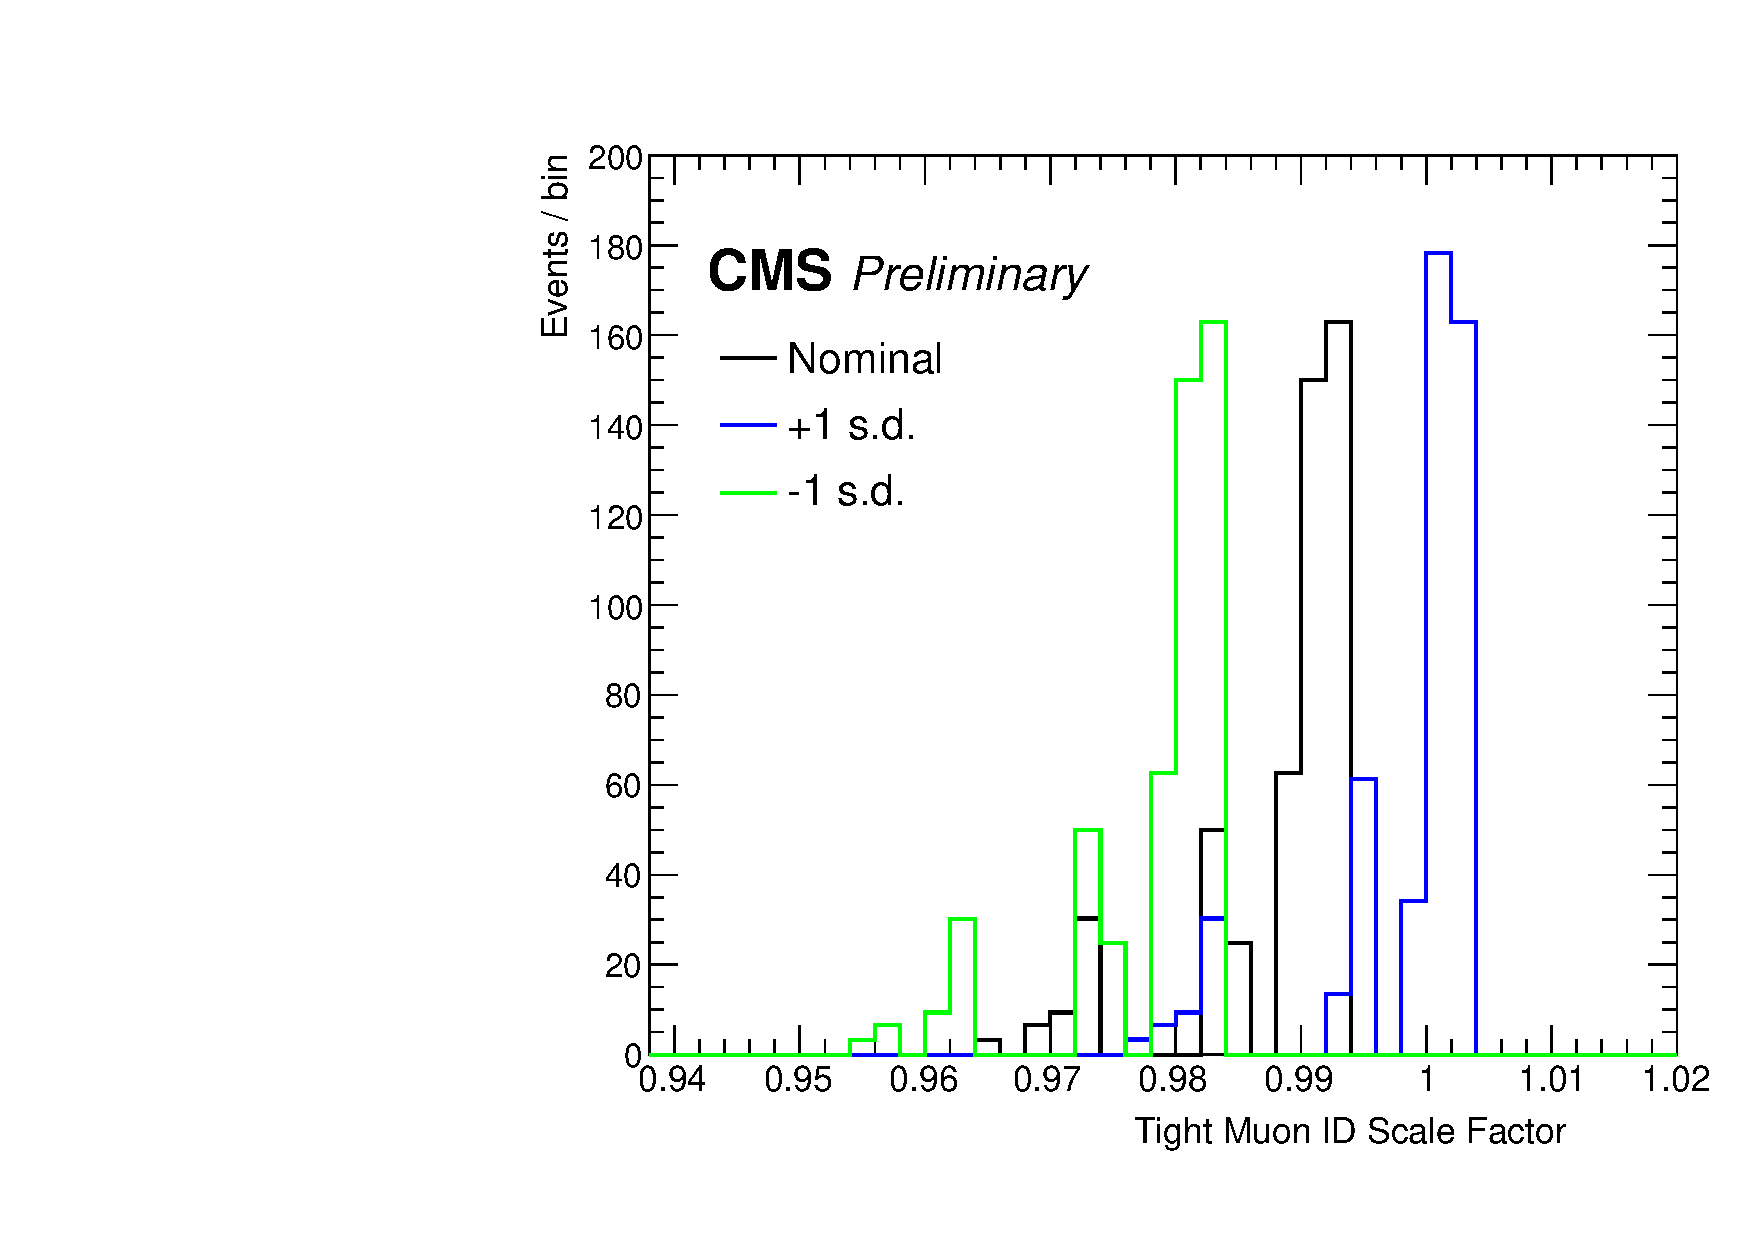
\includegraphics[width=0.45\textwidth]{figures/idSF.pdf}
        \hspace{0.01\textwidth}
        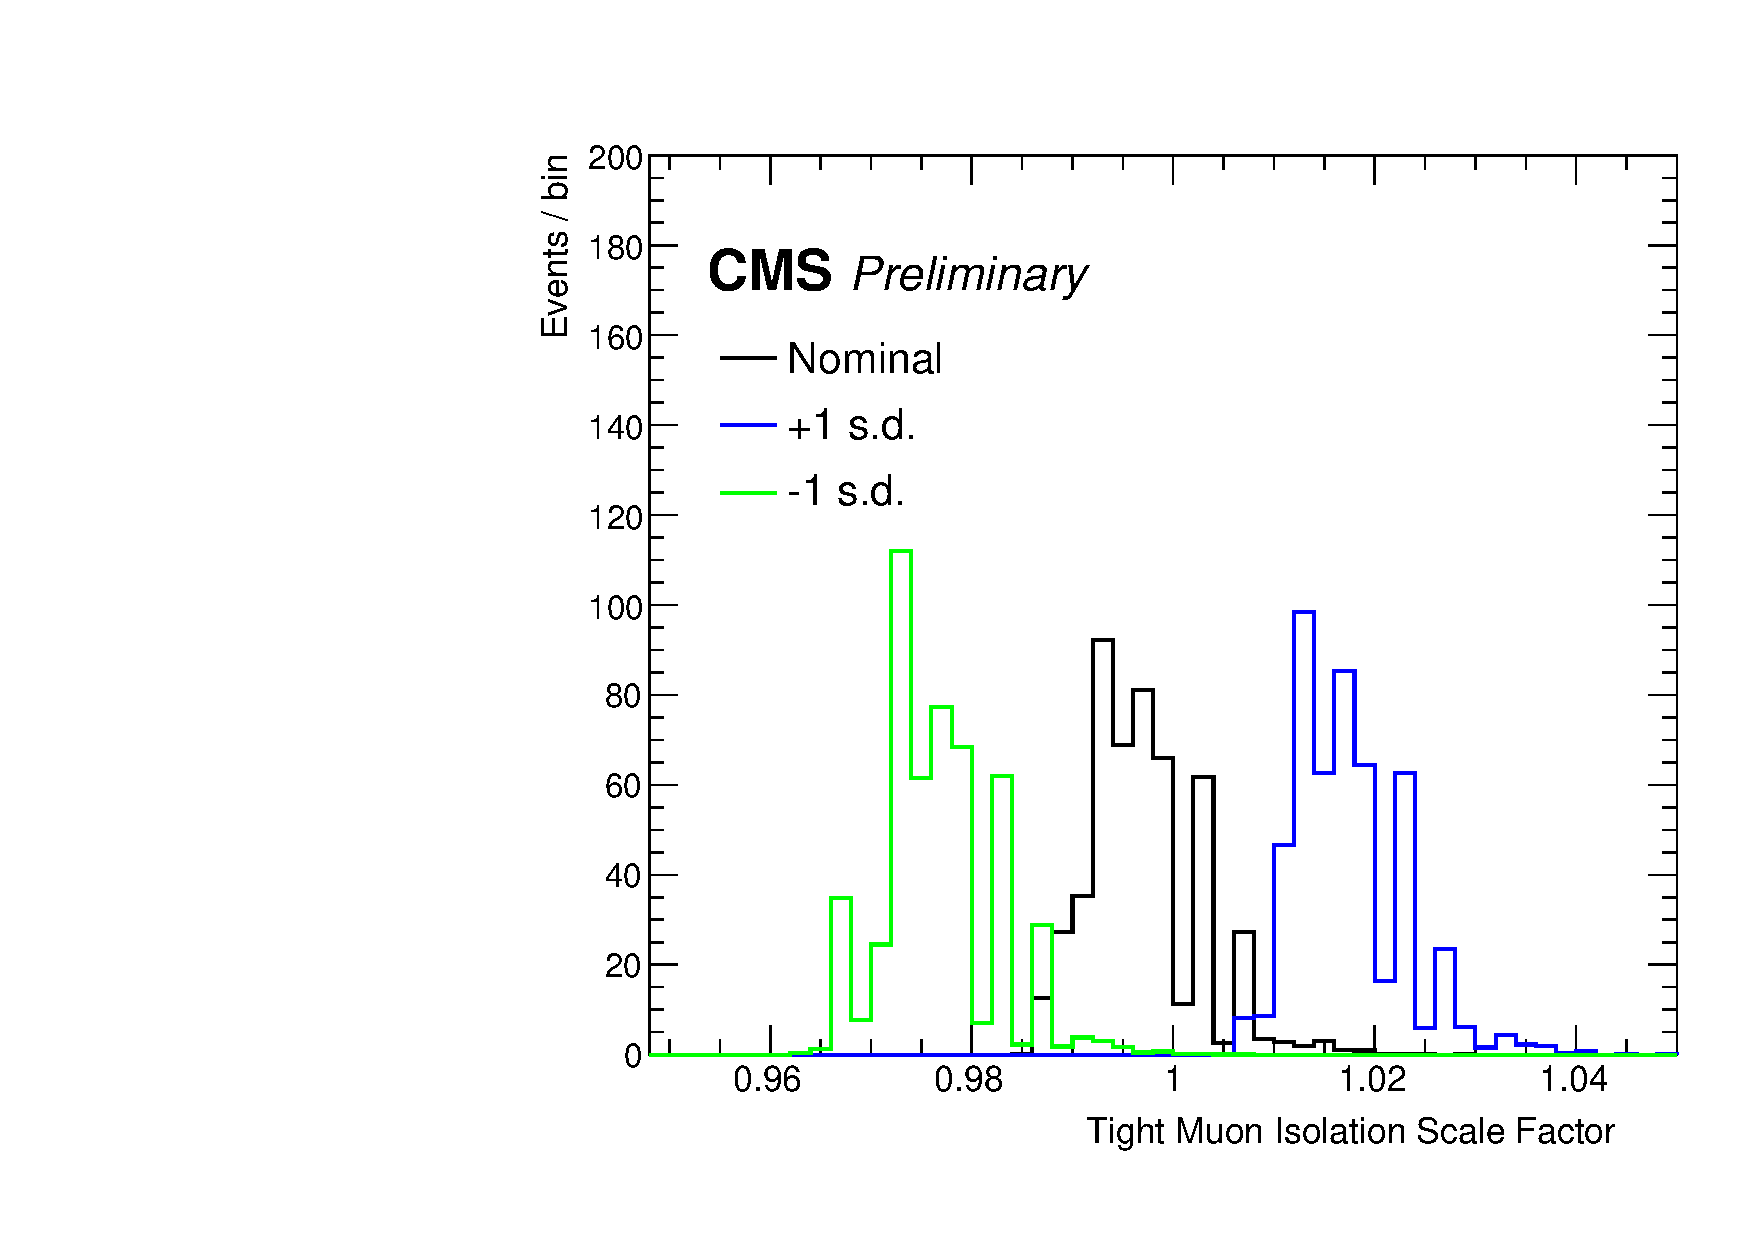
\includegraphics[width=0.45\textwidth]{figures/isoSF.pdf}
	\caption[Muon ID and Isolation Scale Factors]{The Muon ID and Isolation scale factors applied to the simulated DY events, calculated using the $\eta$ and $p_t$ of the tagging muon.}
        \label{fig:muIdIsoSFs}
\end{figure}

The efficiency of the isolated muon triggers used in this search are corrected using similar tag-and-probe techniques as the identification efficiency. 
By selecting events with high-quality tagging muons which pass the trigger requirements and selecting probe muons with reduced identification requirements, the rate of muons with particular $\eta$, $\pt$, and isolation passing the trigger can be compared in data and MC.

All MC events are then applied a weight based on the relative rate of their tagging muons passing the trigger in data and MC, and a systematic uncertainty in this trigger efficiency is applied by changing the trigger efficiency by one standard deviation.
To ensure that this efficiency is calculated for the correct muon, all tagging muons selected are required to pass the isolated muon trigger used in this search.

\subsection{Muon Energy Scale Corrections}
While this analysis has a weak overall sensitivity to the tagging muon kinematics, small differences that may be present between simulation and data in the tagging muon energy could cause shifts in the invariant mass distribution which change the event acceptance rate.
Simulated bias effects which are asymmetric in charge, such as mismodelling of the magnetic field, could also introduce bias into the expected charge distribution of the selected probe tracks.
To account for these potential differences, muon energy scale corrections are applied using the Rochester method \cite{rochester_corr}.

The Rochester method is a data-driven correction to reconstructed muon energies as a function of $\eta$, $\phi$, and charge.
The correction is derived using a two-step approach which uses $Z/\gamma* \rightarrow \mu\mu$ events.
In the first step, DY events are generated for a perfectly aligned detector by smearing the generator level momentum using a function that replicates the experimental resolution as a function of $\eta$. 
Corrections for both data and MC are then derived by requiring that the average $1/p_t^\mu$ of muons from Z decays matches the perfectly-aligned MC.

In the second step, further corrections are derived for each $\eta-\phi$ bin so that the reconstructed Z mass is the same as the perfectly aligned detector. 
This step removes scatter in average Z mass which can result from the first step due to variations in muon efficiency between $\eta-\phi$ bins that are not perfectly modeled in MC. 
The muon energy scale corrections are applied to all tagging muons, and uncertainties in the resulting muon momentum are included as an overall systematic based on the change in signal efficiency produced when varying them by one standard deviation.

\subsection{HCAL Efficiencies}
\label{sec:HCALeff}
The response of the HCAL to muons is important in this study to reject events with large energy deposits as well as events where the selected probe did not reach the calorimeters.
In addition, the depth-by-depth information can be used to search for evidence of a change in muon energy within HCAL as a signature of a \dbrem.
In order to use this level of detail, the muon HCAL deposits in MC must be validated and corrected to match those seen in data.
This is done through study of muon deposits along the trajectory of selected tagging muons.

As the global muon associated with the tag may have improved trajectory accuracy due to the inclusion of information from the muon systems, the tracker track matching the global muon is projected into HE to match the information available for the selected probes.
The HCAL energy is then collected in each depth along the trajectory of the track, and the distributions of energy are compared in data and DY MC. 

Initial studies of the muon energy deposits found significant excesses in data of depths with less than \SI{0.1}{\giga\eV}, referred to as 'missing' hits (\Cref{fig:missingHits}. 
Study of these events found that events with many missing hits correspond to probe trajectories that align with the edges of HE cells (\Cref{fig:cellEdges}), and are likely caused by a combination of effects from differences in light collection efficiency with particle position that are not replicated in simulation, gaps between cells causing small regions of missing coverage, and misalignment between the CMS tracker and HCAL in reconstruction.

\begin{figure}[ht]
	\centering
	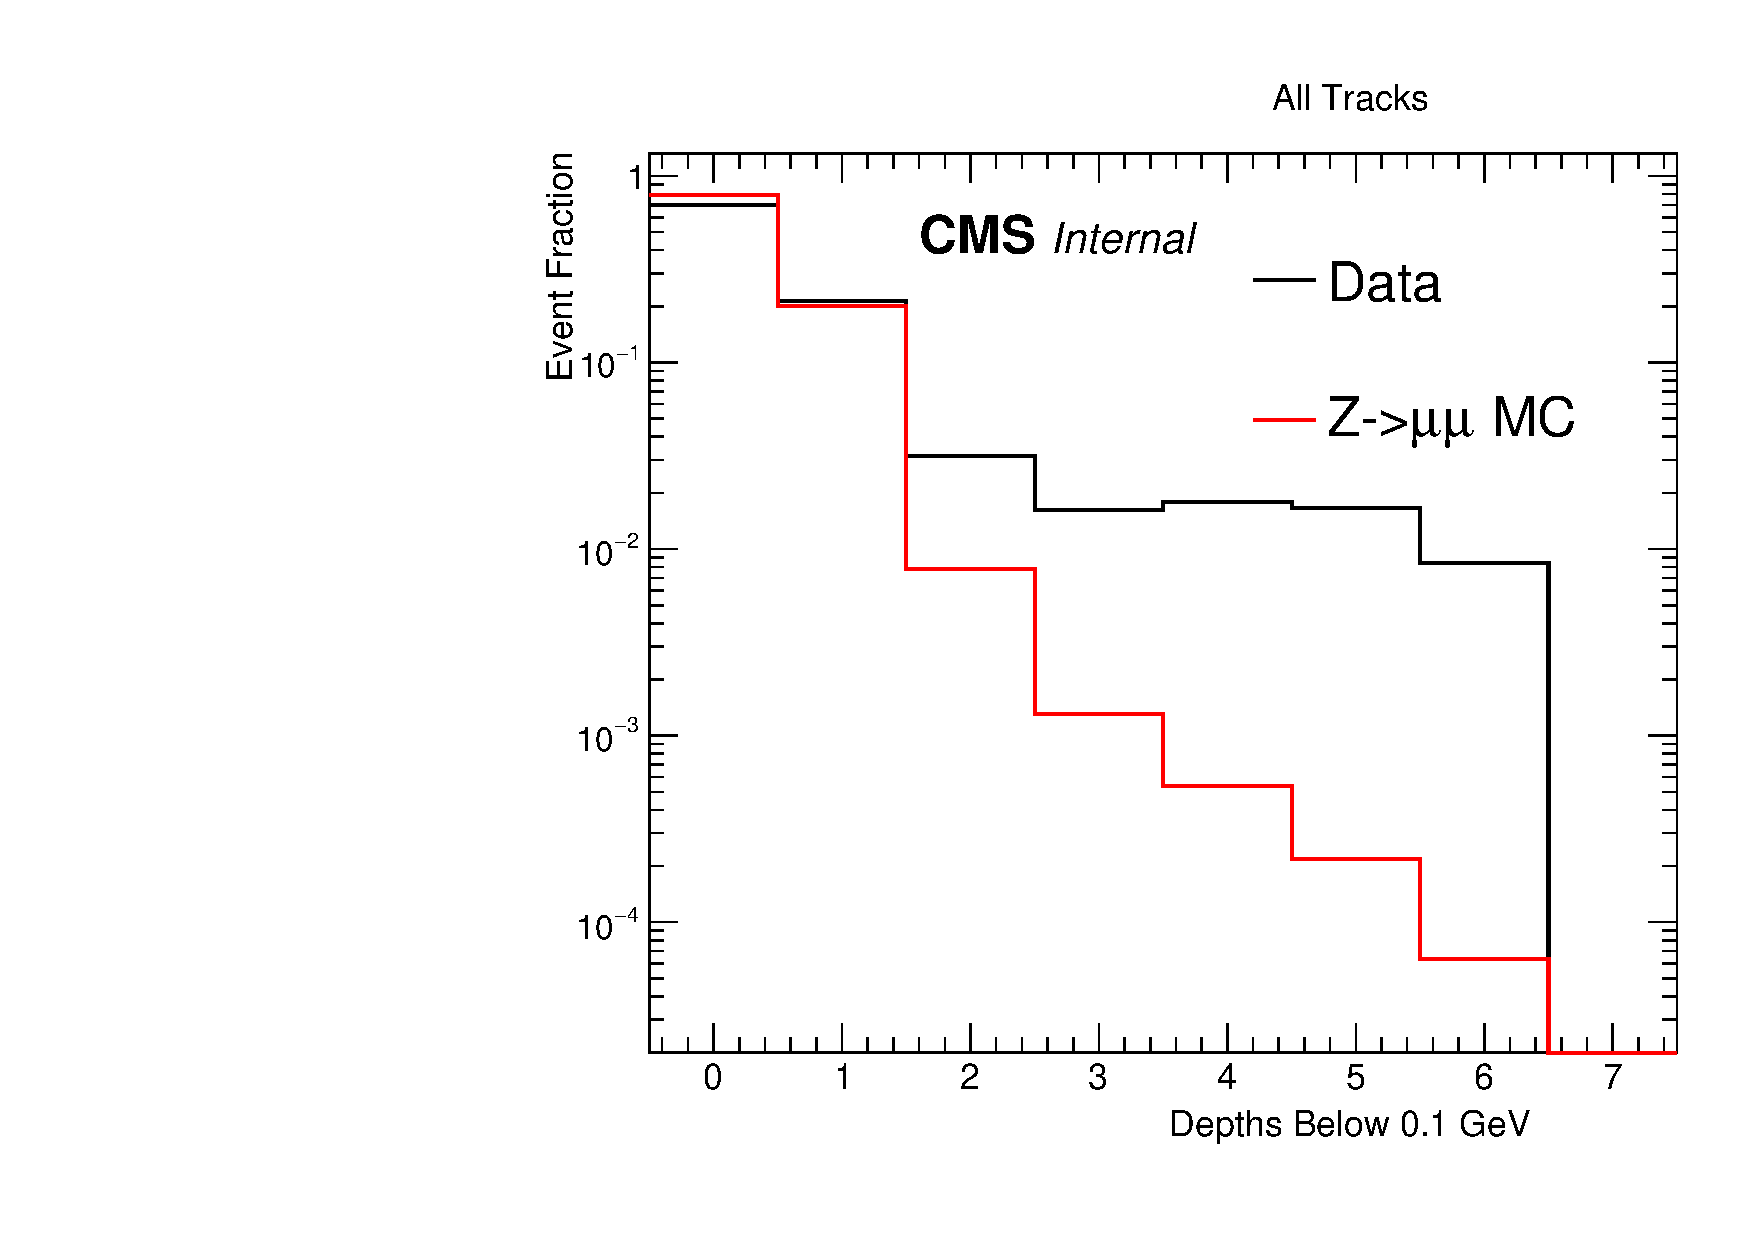
\includegraphics[width=0.45\textwidth]{figures/hcalAllMissingHits.pdf}
        \hspace{0.01\textwidth}
        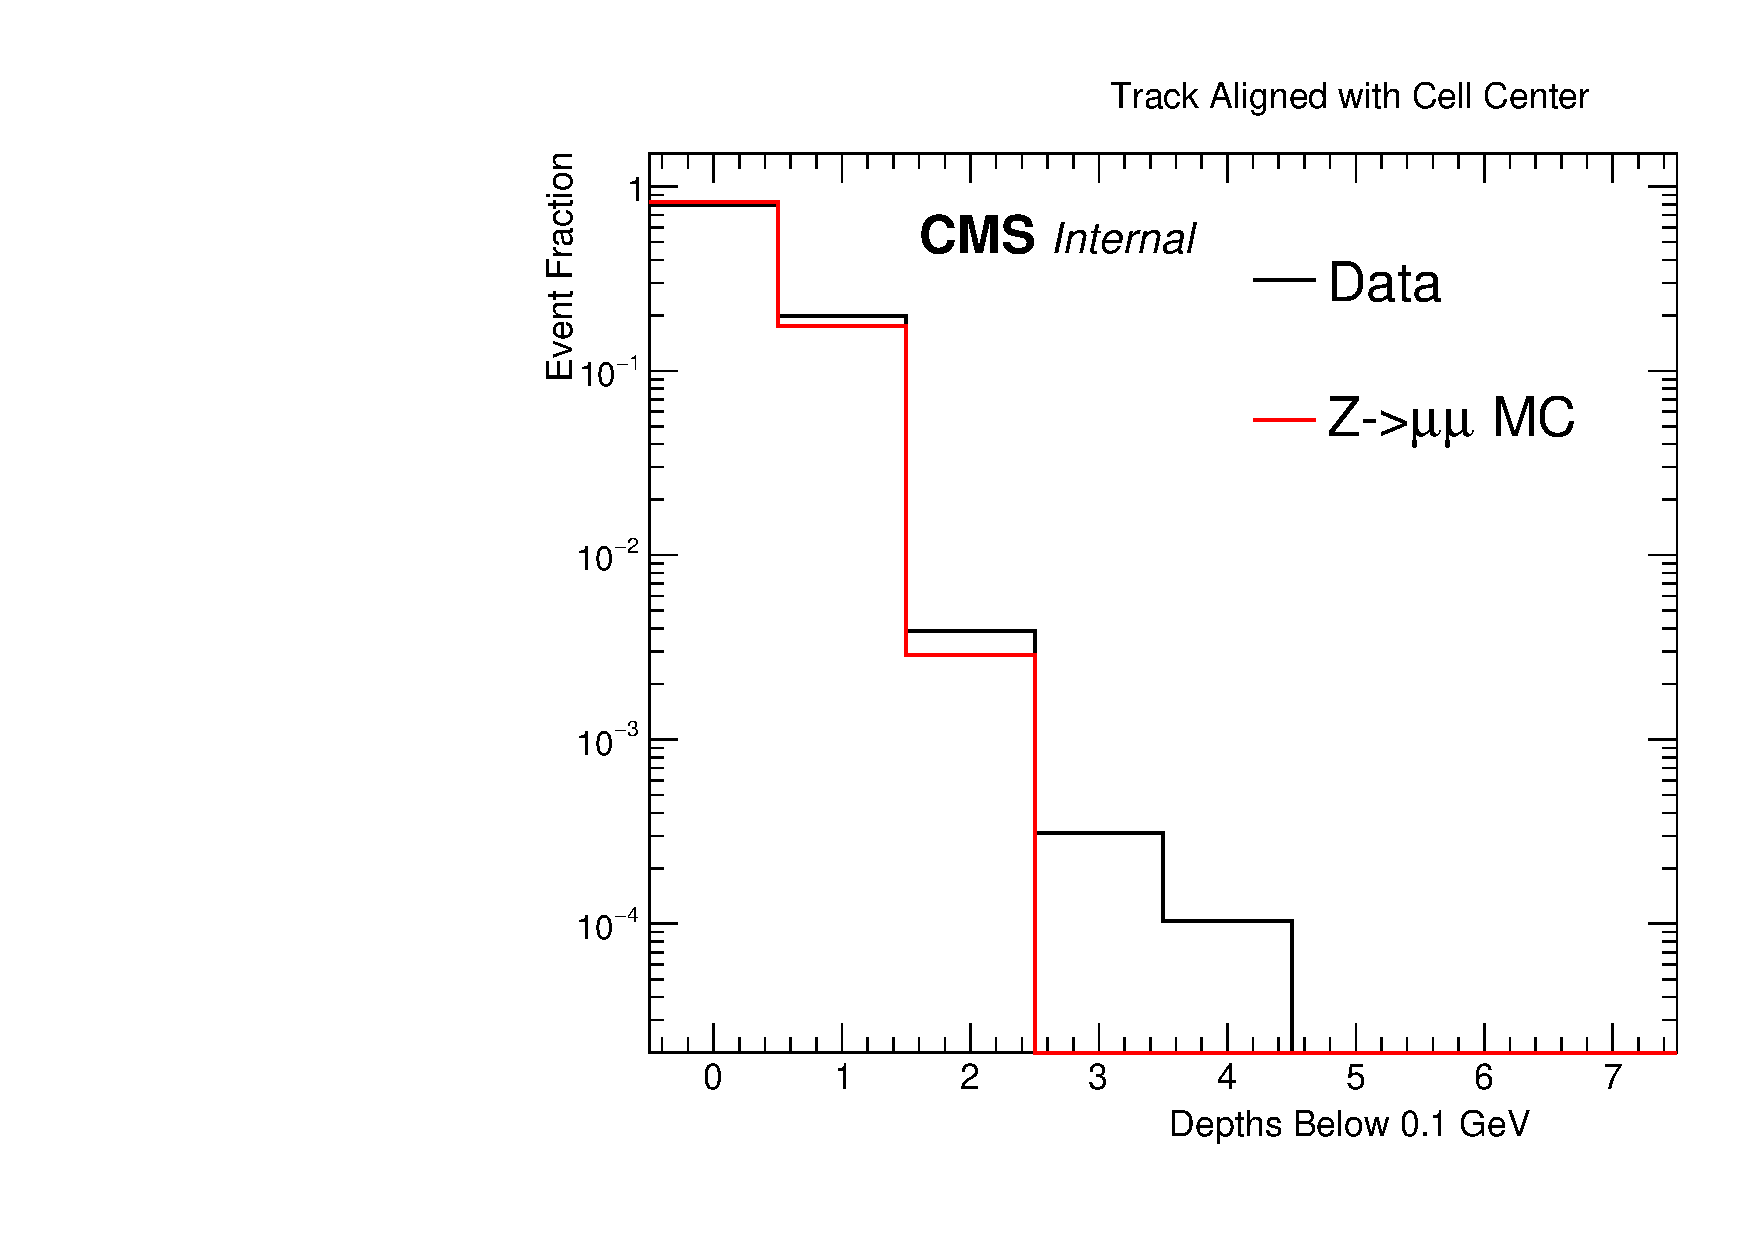
\includegraphics[width=0.45\textwidth]{figures/hcalMissingHits.pdf}
        \caption[Missing muon hits in HE]{The number of HE depths along tagging muon trajectories below \SI{0.1}{\giga\eV} for all selected muons (left) and for those not near HE cell edges (right). Significant excess in events with many missing hits is seen in data events with tracks near cell edges.}
        \label{fig:missingHits}
\end{figure}

\begin{figure}[ht]
	\centering
	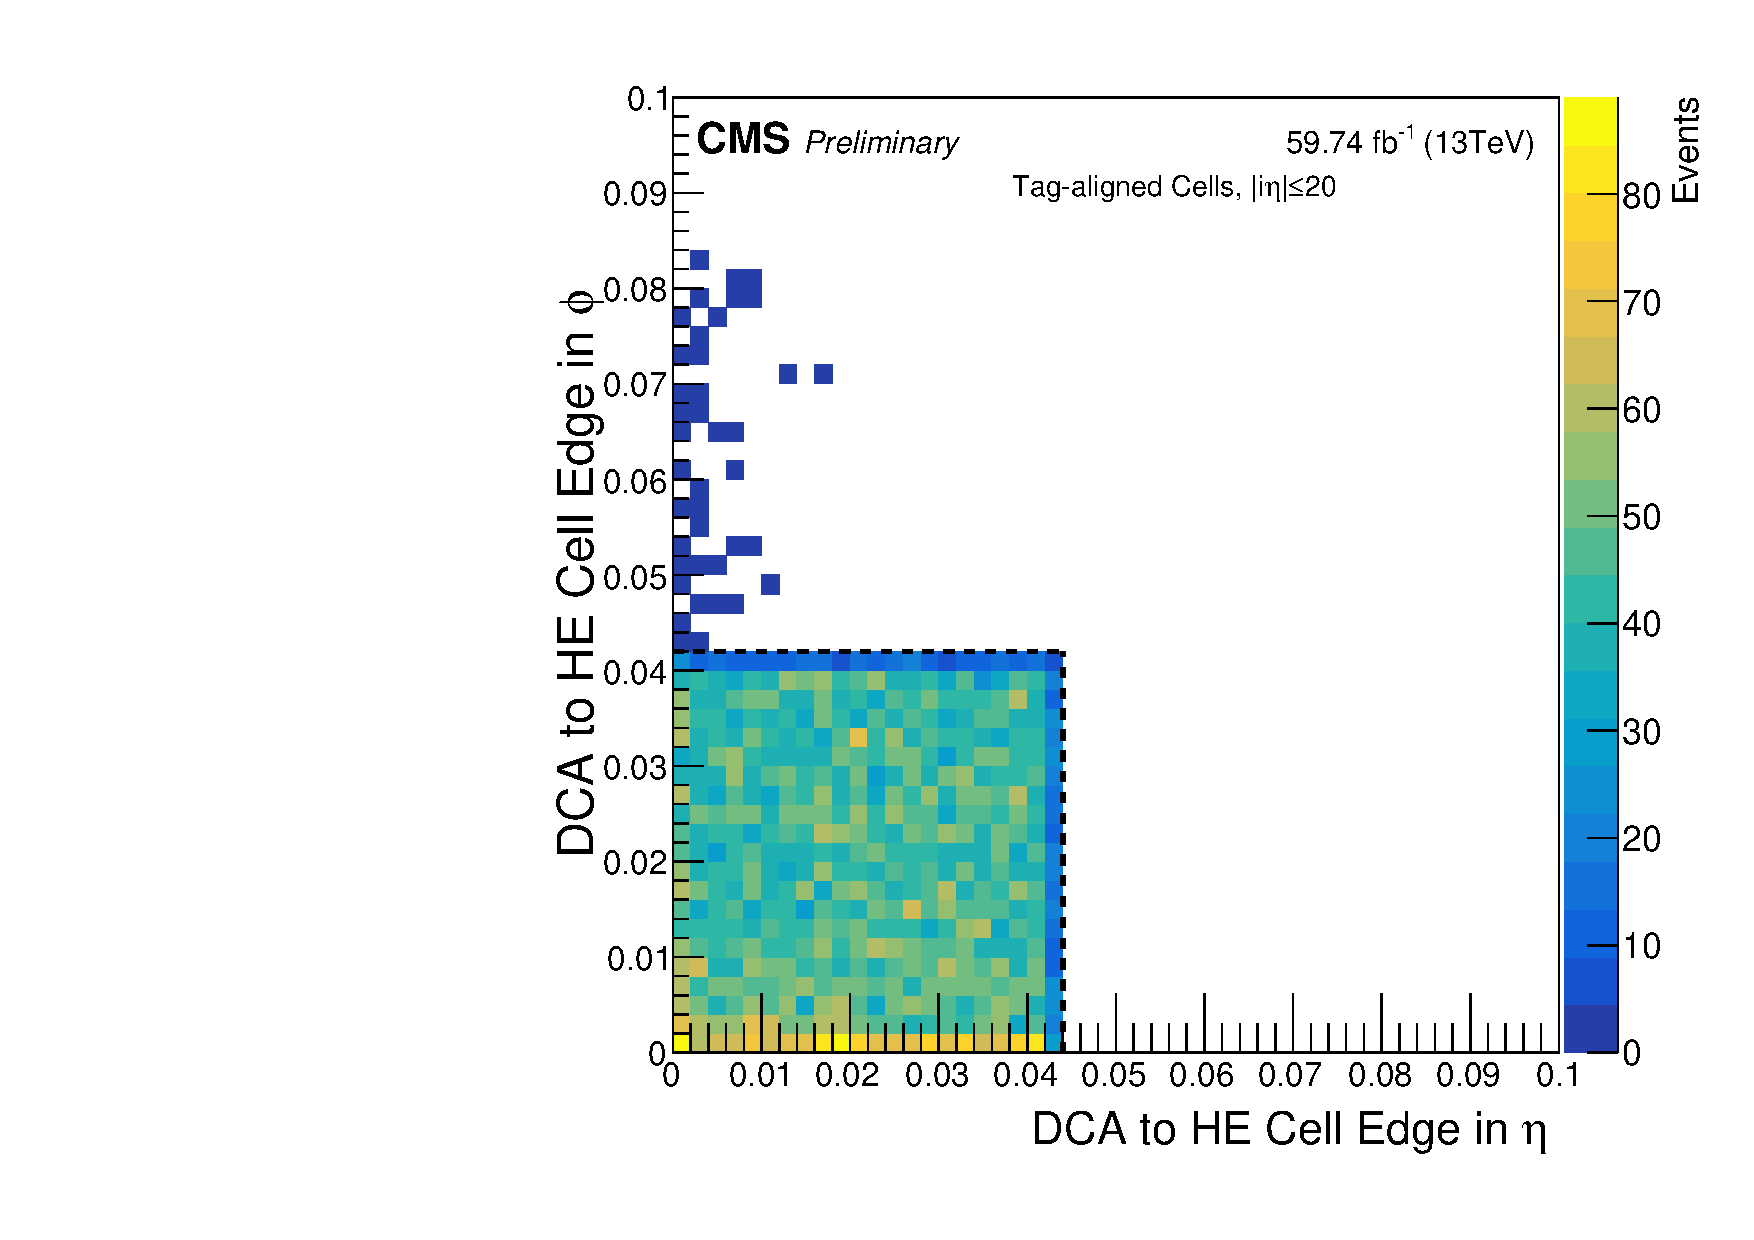
\includegraphics[width=0.45\textwidth]{figures/HEEdgeDistance_all_smallCell.pdf}
        \hspace{0.01\textwidth}
        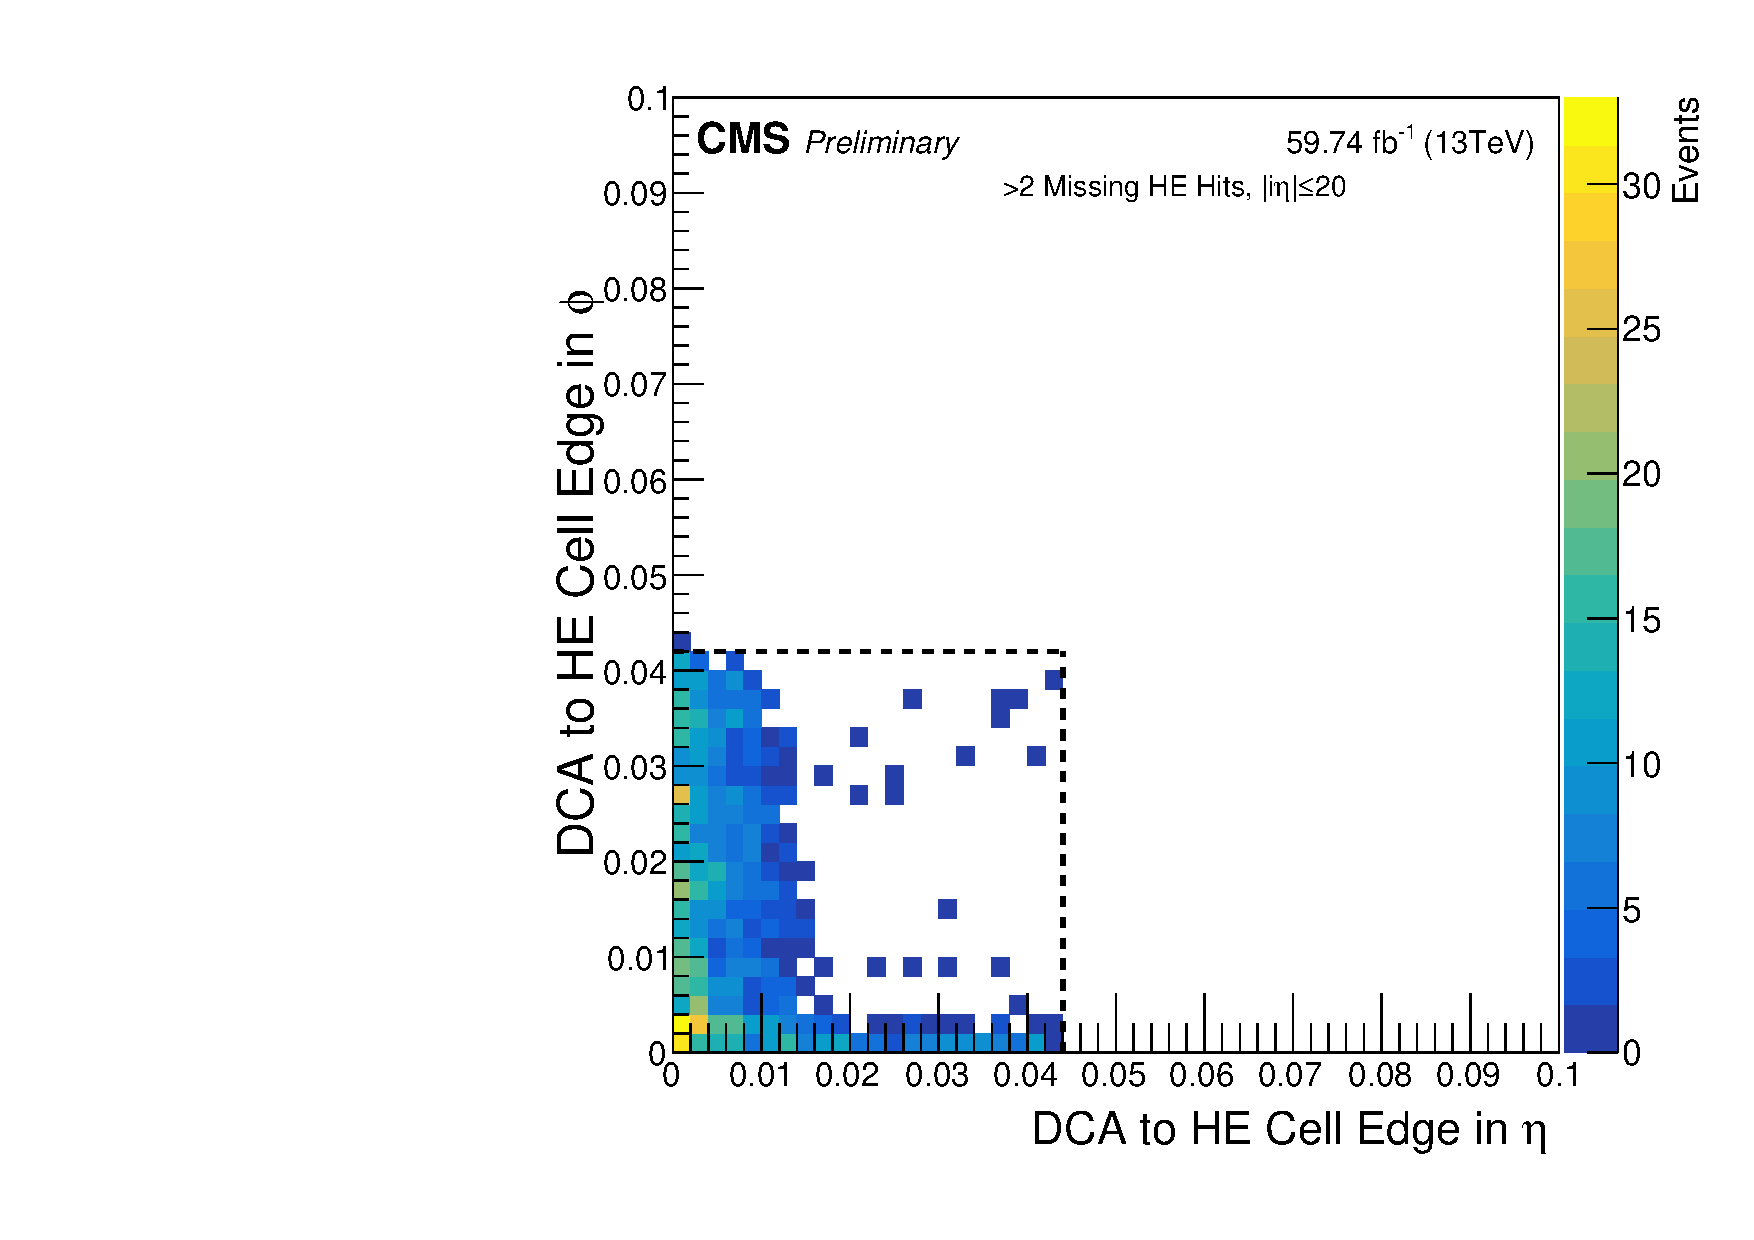
\includegraphics[width=0.45\textwidth]{figures/HEEdgeDistance_multMissing_smallCell.pdf}
	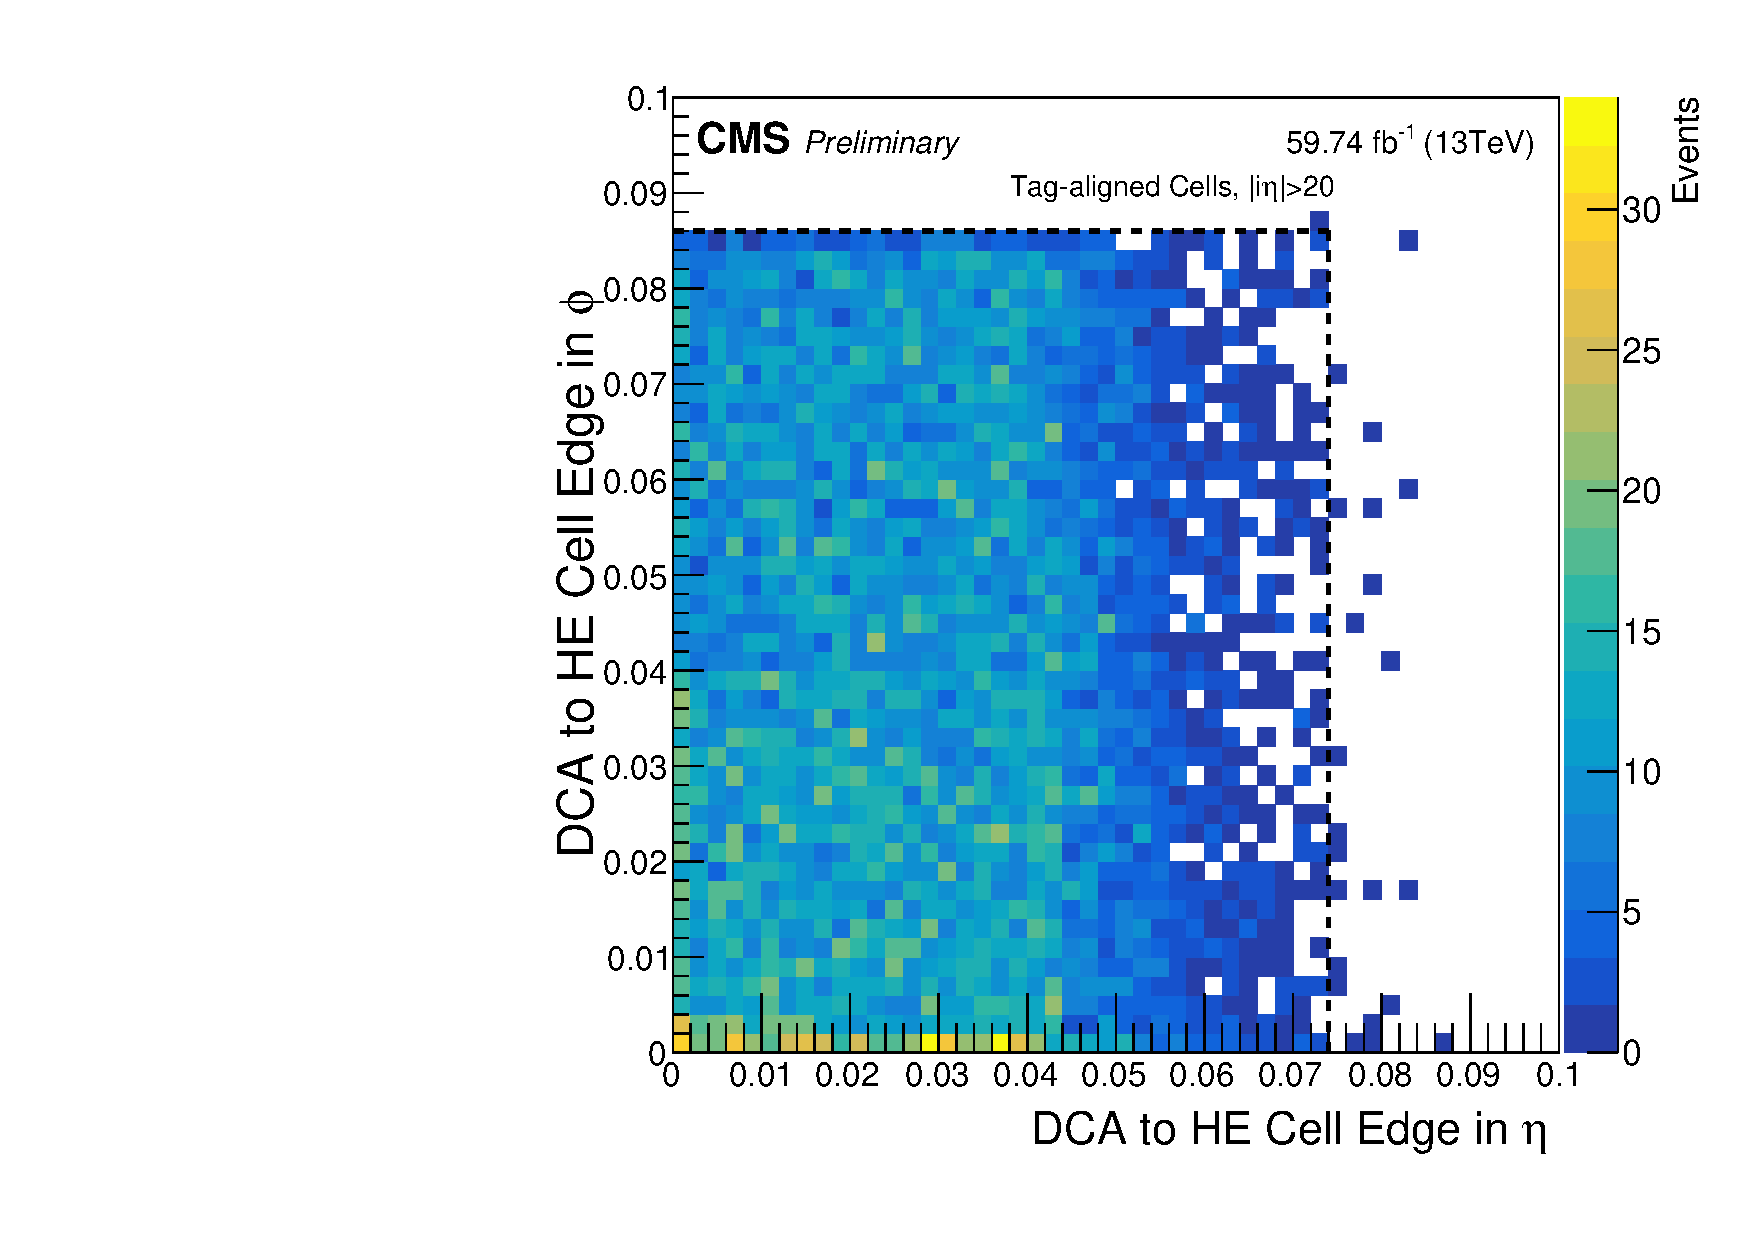
\includegraphics[width=0.45\textwidth]{figures/HEEdgeDistance_all.pdf}
        \hspace{0.01\textwidth}
        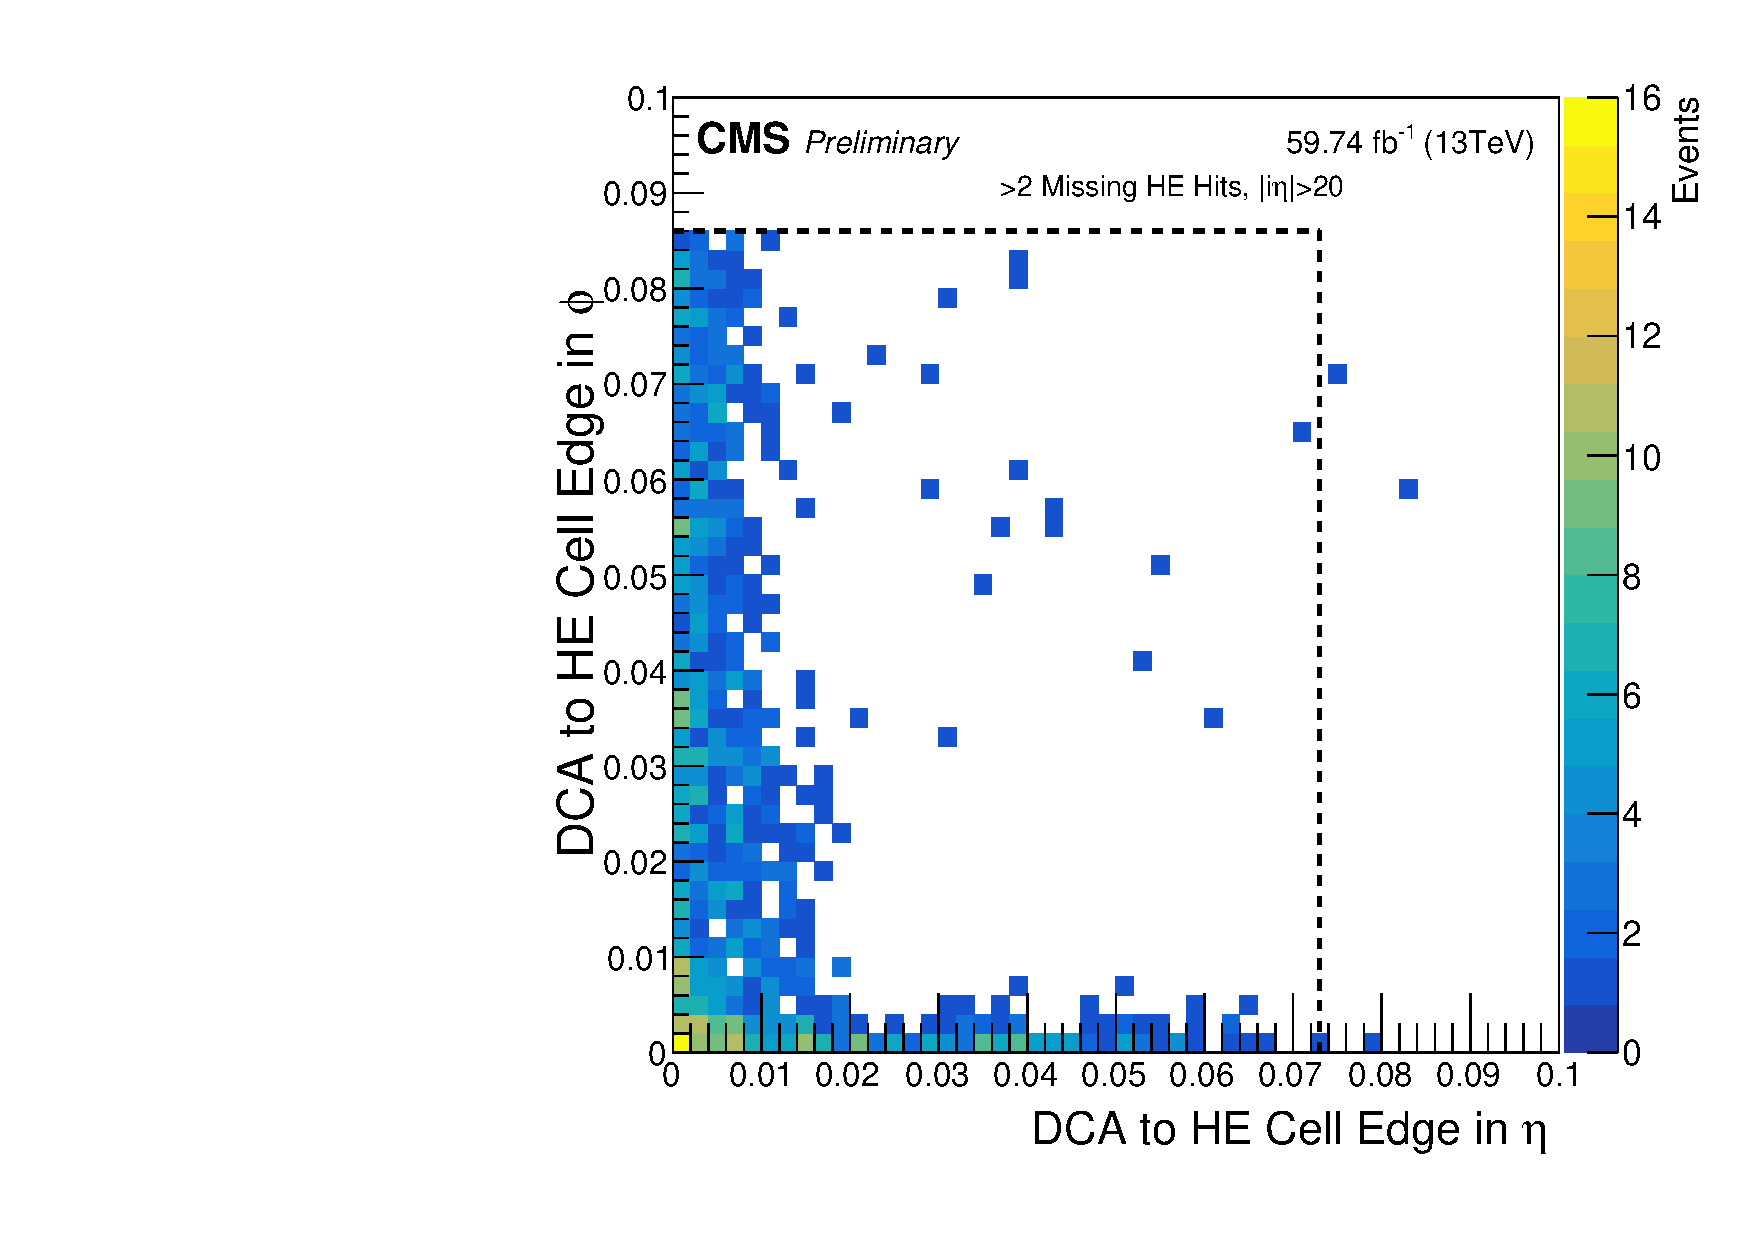
\includegraphics[width=0.45\textwidth]{figures/HEEdgeDistance_multMissing.pdf}

        \caption[Muon distances to HE cell edges]{The distance of closest approach (DCA) to any HE cell edge for tagging muons used to validate HE hits. Events with more than two missing hits (right) are clustered near the edges of HE cells, while the overall distribution of tracks is spread evenly across the cell size. The vertical splitting reflects the two different cell sizes in the detector, although the cell size is not observed to significantly change the size of the regions with many missing hits.}
        \label{fig:cellEdges}
\end{figure}

Anomalous low-hit events that are produced by misalignment between the HE and the tracker in reconstruction will have correlations between the probe track trajectory and the $\Delta\eta$ and $\Delta\phi$ to cell edges which produce significant missing hits. 
To study these correlations, the $\eta$ edge and $\phi$ edge events are first categorized using requirements of |$\Delta\phi$| $<$0.004 a |$\Delta\eta$| $<$0.016, respectively. 
By defining tag-aligned probe track data events which are not near $\phi$ edges as well as similar tag-aligned events which are not near $\eta$ edges, the two patterns can be separated and correlations in the cell edge distances which produce many missing hits and the probe track trajectory can be found. 
The minimum $\Delta\phi$ in non-$\eta$-edge events with multiple missing hits is shown as a function of $\phi$ in \Cref{fig:phiEdgeCorr}, and the minimum $\Delta\eta$ in non-$\phi$-edge events with multiple missing hits is shown as a function of $\eta$ for both endcaps in \Cref{fig:etaEdgeCorr}.

\begin{figure}[htpb]
    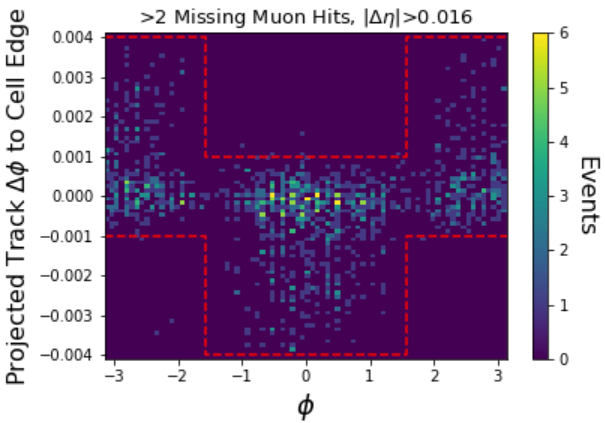
\includegraphics[width=0.45\textwidth]{figures/phiEdgeEventsData.png} 
    \centering
	\caption[$\phi$ edge correlations in missing HCAL muon hits.]{The minimum $\Delta\phi$ to any HE cell edge and the probe track $\phi$ trajectory for tag-aligned probe tracks with multiple missing hits. A sinusoidal dependence on the region with significant missing hits is observed, which is consistent with a relative shift in y between the HCAL and the tracker between data and reconstruction. The region outlined with a dashed red line indicates 'on-edge' events in $\phi$.}
    \label{fig:phiEdgeCorr}
\end{figure}

\begin{figure}[htpb]
    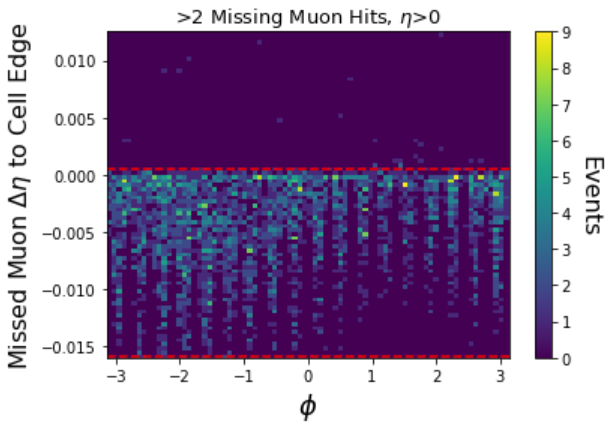
\includegraphics[width=0.45\textwidth]{figures/posEtaEdgeEventsData.png} 
    \hspace{0.01\textwidth}
    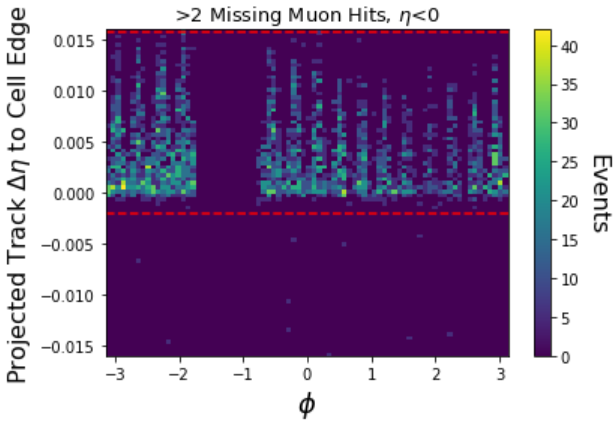
\includegraphics[width=0.45\textwidth]{figures/negEtaEdgeEventsData.png}
    \centering
	\caption[$\eta$ edge correlations in missing HCAL muon hits.]{The minimum $\Delta\eta$ to any HE cell edge and the probe track $\phi$ trajectory for tag-aligned probe tracks with multiple missing hits in the positive (left) and negative (right) HCAL endcaps. The events with multiple missing hits have a strong dependence on the sign of $\Delta\eta$ to the missing cell edges. The regions outlined with dashed red lines indicate 'on-edge' events in $\eta$.}
    \label{fig:etaEdgeCorr}
\end{figure}

To accounting for these correlations, the 'on-edge' requirements are chosen to be dependent on the probe track trajectory as well as the cell edge distance. 
Probe tracks are designated as on-edge in $\eta$ if -0.002$<\Delta\eta<$0.016 and the probe track trajectory has $\eta<0$, or if -0.016$<\Delta\eta<$0.002 and the probe track trajectory
has $\eta>0$.
Probe tracks are designated as on-edge in $\phi$ if -0.001$<\Delta\phi<$0.004 and the probe track trajectory has $|\phi|>\pi/$2, or if -0.004$<\Delta\phi<$0.001 and the probe track trajectory has $|\phi|<\pi/$2.

Events which are on-edge in $\eta$, $\phi$, or both are excluded from the partial disappearance region due to the significant differences observed between data and MC in the individual HE hits, which are necessary in that region to remove soft SM Bremsstrahlung backgrounds.
In complete disappearance events, the HCAL hits are implemented using sums of all HCAL cells within a $\Delta$R cone of 0.3, which is sufficiently large to include all adjacent cells and so does not have visible differences due to this misalignment.

After removing the on-edge events, small variations in the energy of muons in HE are still observed. 
To correct for these differences, event weights are derived for each depth in HE as a function of the energy in that depth based on the difference observed between DY MC and data.
Additionally, to avoid potential differences in the simulated zero-suppression thresholds which may cause significant changes in events with very low HE energy, all HE hits with reconstructed energy below \SI{0.1}{\giga\eV} are set to zero.

\subsection{Pileup Correction}
Generation of simulated events generally occurs during the data taking period, when the exact pileup distribution is not well known.
As a result, estimates of the distribution of pileup vertices are used during the initial MC generation. 
After data taking is complete and the resulting pileup distribution is measured, the simulated events are re-weighted to recreate the observed pileup.
Pileup events may produce particles which are mistakenly identified as muons or are in the vicinity of a probe track and cause it to fail isolation requirements, so potential differences in the number of pileup particles between data and MC could impact the expected signal strength.

To perform this re-weighting, histograms of the amount of pileup observed in data are divided by those used to generate the MC samples to find the weight for each potential number of pileup interactions (\Cref{fig:pileup}).
The number of pileup interactions used for this re-weighting is not directly the number of pileup vertices in the event, which is dependent on the vertex reconstruction efficiency in the event and can introduce large systematic errors and biases.
Instead, the rate of pileup is determined from the product of the total inelastic pp cross section in CMS and the instantaneous luminosity, defined as the luminosity measured over each 23 second period ("lumisection") in CMS.
The amount of pileup in each event is then found by dividing this rate by the collision frequency.

As a result of this process, the measured pileup has a systematic uncertainty produced by uncertainty on the measured total pp inelastic cross section as well as the instantaneous luminosity. 
These effects are included as a pileup re-weighting uncertainty by varying the product of cross section and luminosity by one standard deviation in each direction.
For the pileup calculation, the nominal total inelastic cross section of $\sigma_{pp}=$\SI{69.2}{\milli\barn} was used with an overall uncertainty of $\pm4.6\%$\cite{pileupCx}.

\begin{figure}[ht]
	\centering
	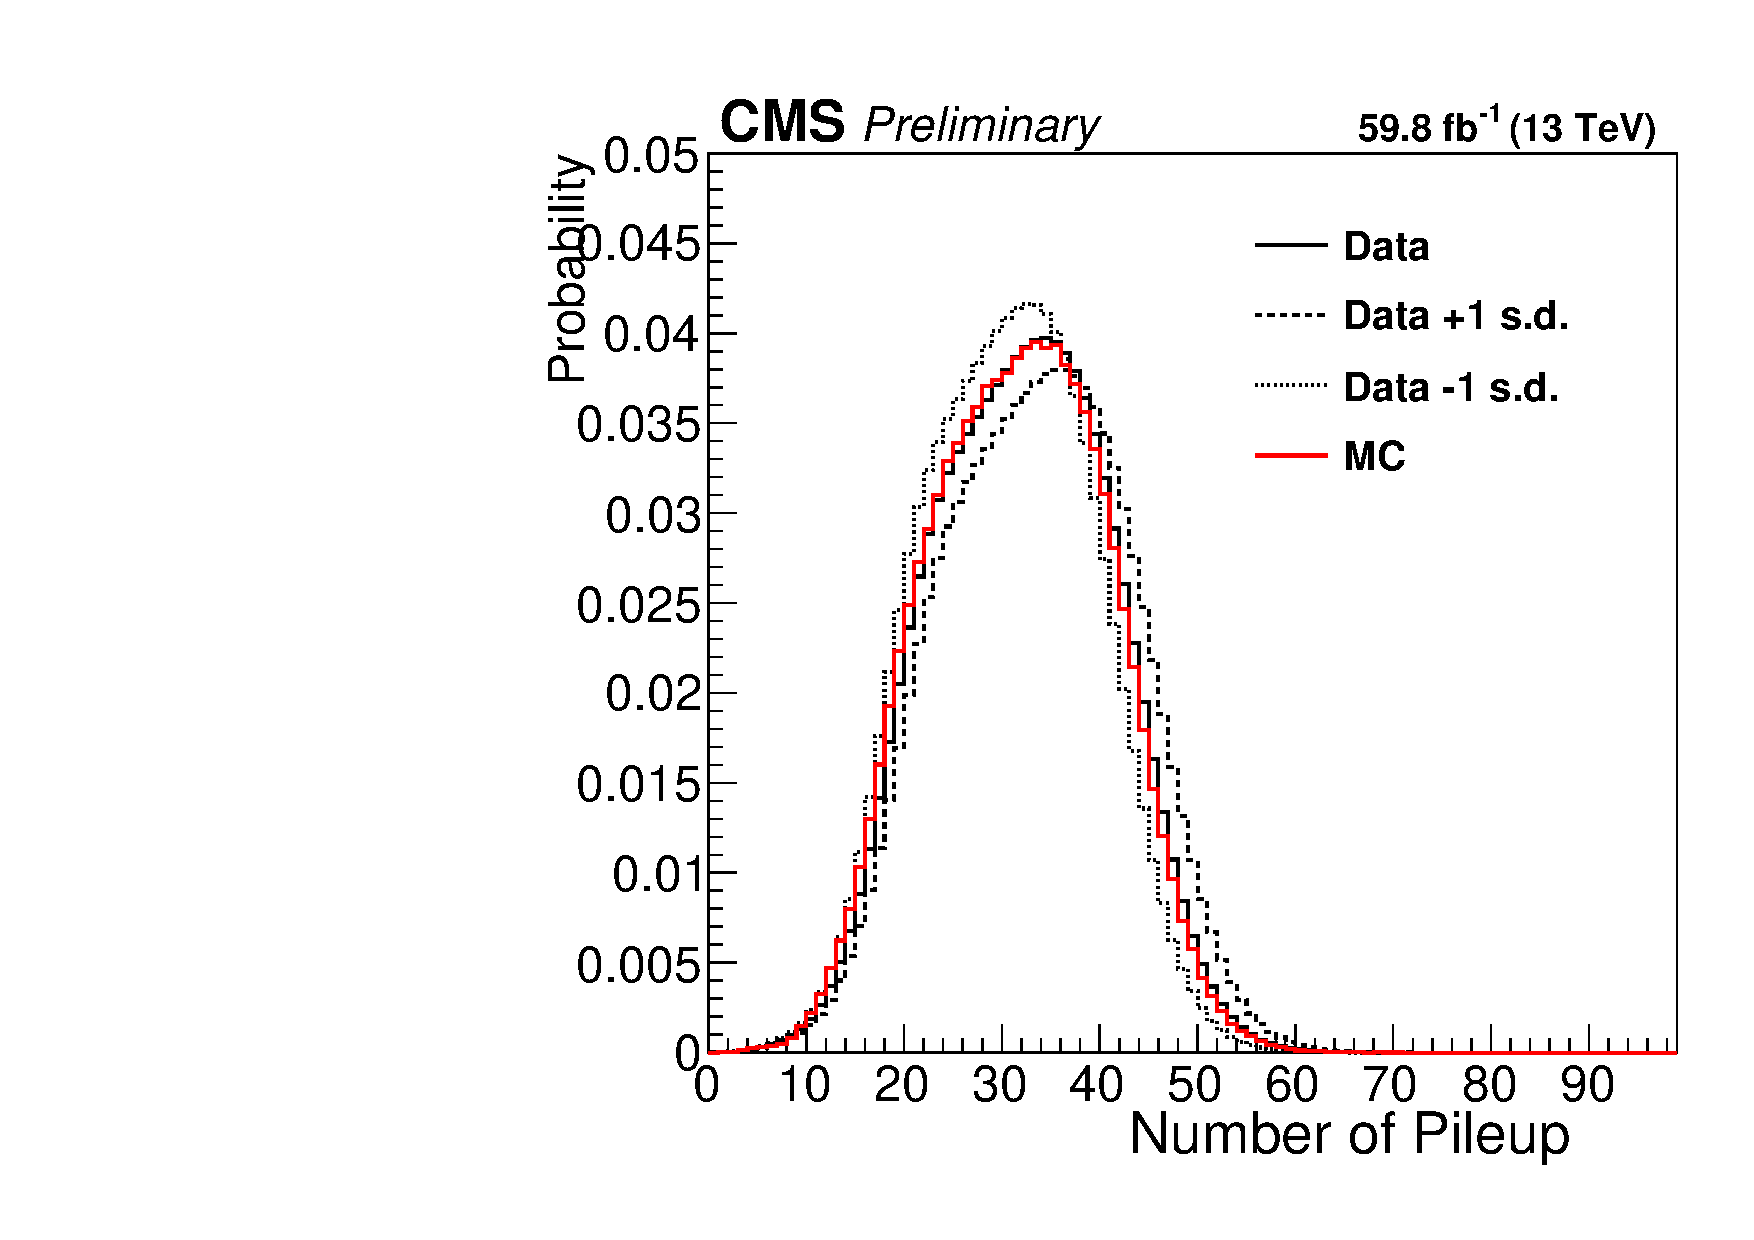
\includegraphics[width=0.45\textwidth]{figures/PileupDists.pdf}
	\hspace{0.01\textwidth}
	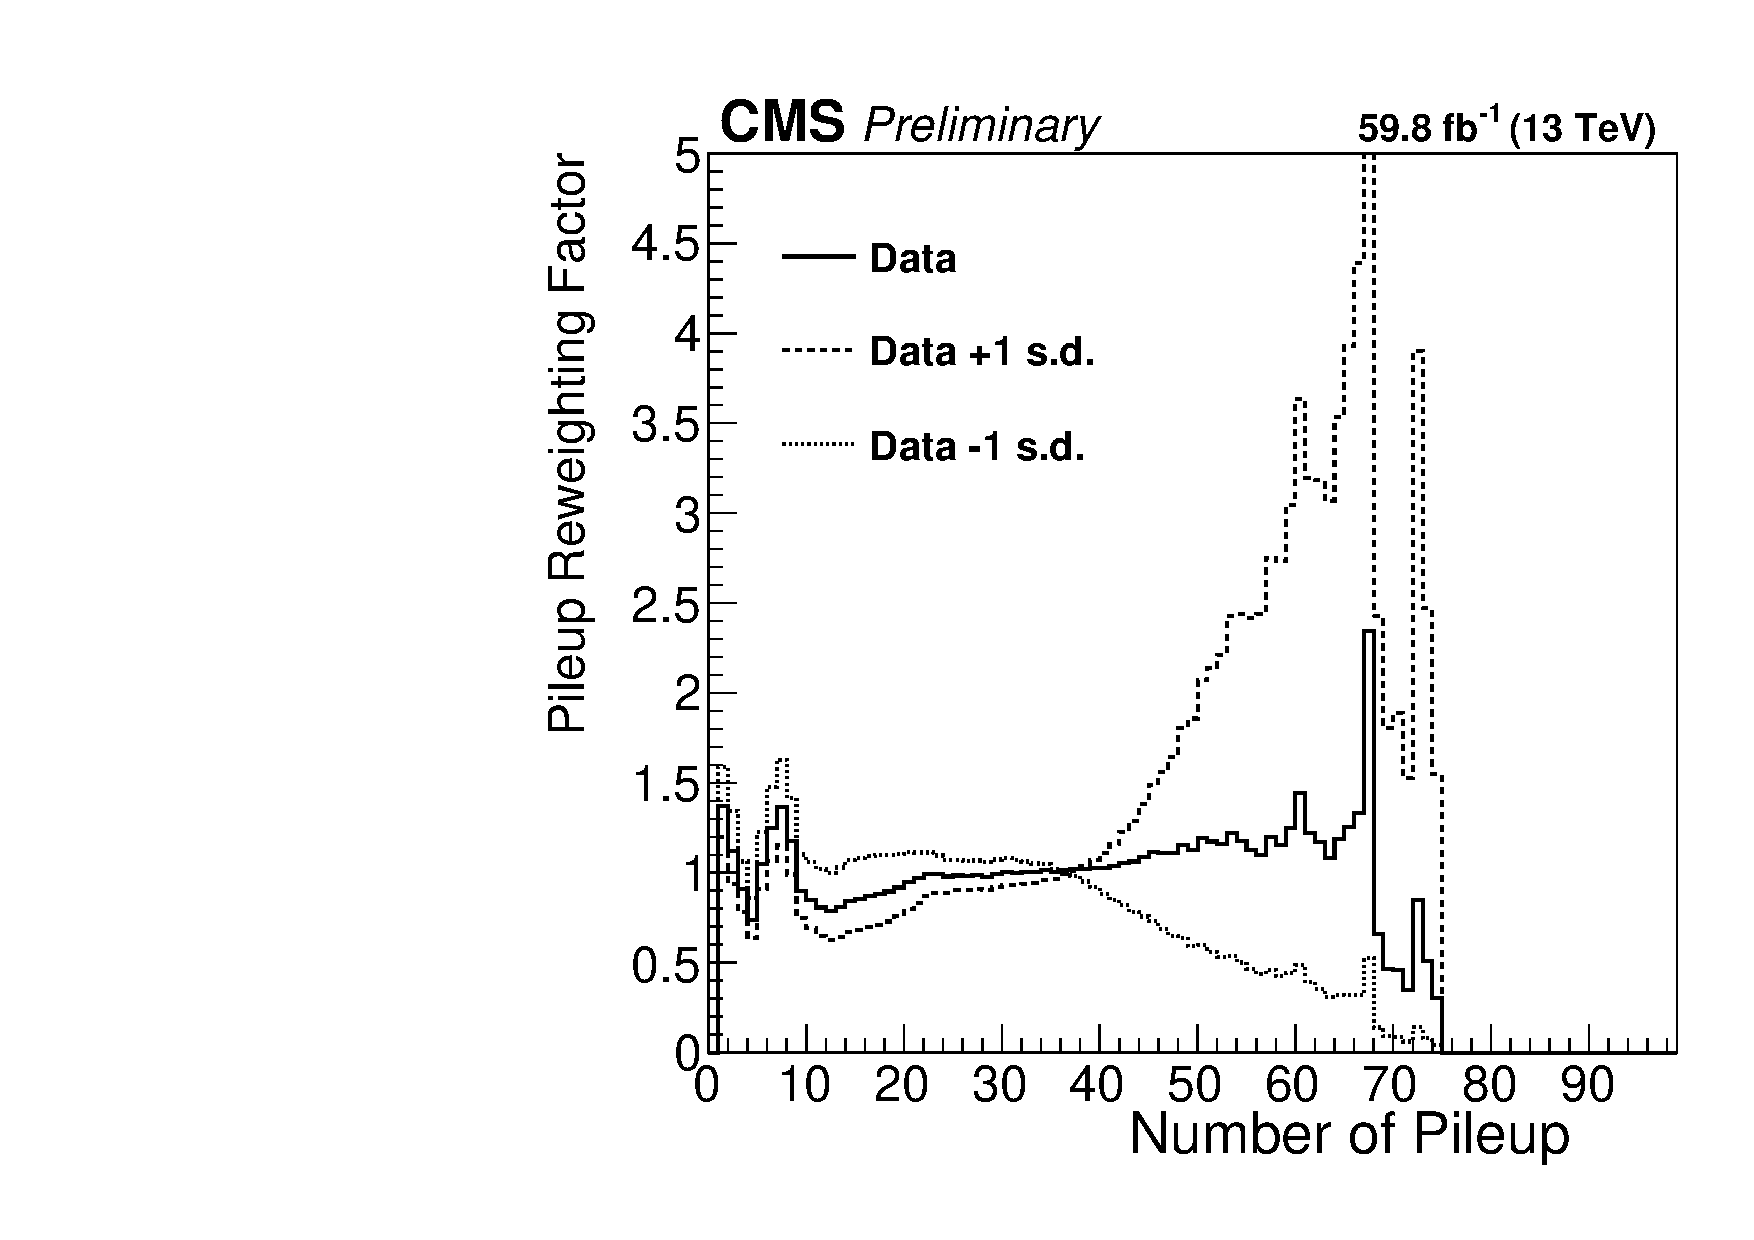
\includegraphics[width=0.45\textwidth]{figures/PileupRatioDists.pdf}
        \caption[Pileup Re-weighting Histograms]{The number of pileup interactions (left) and the pileup re-weighting factors (right) derived from their ratio.}
        \label{fig:pileup}
\end{figure}

%%%%%%%%%%%%%%%%%%%%%%%%%%%%%%%%%%%%%%%%%%%%%%%%%%%%%%%%%%%%%%%%%%%%%%%%%%%%%%%%
